%% Pedersen hash implementation standard %%

% TELL THEM: These are things we are improving, so it is a draft. Let me know if there is anything else I should add.
% B-JJ vs. B JJ

\documentclass[11pt]{article}
\usepackage[colorlinks=true,
			urlcolor=black,
			linkcolor=black,
			citecolor=black
			]{hyperref} 
\usepackage[parfill]{parskip}

\usepackage[english]{babel}
\usepackage[utf8]{inputenc}
\usepackage{amsmath, amsthm, amssymb}
\usepackage{enumerate, enumitem}
\usepackage{graphicx}
\usepackage{color, xcolor}
\usepackage{setspace}
\usepackage{hyperref}
\usepackage{authblk}
\usepackage{tikz}
\usetikzlibrary{arrows}
\usetikzlibrary{positioning}
\usepackage{mathtools}
%floor vs. ceil
\DeclarePairedDelimiter{\floor}{\lfloor}{\rfloor} 
\DeclarePairedDelimiter{\ceil}{\lceil}{\rceil}  % If called \ceil*{x} it will add left/right.

%\usepackage{algorithmicx}
\usepackage{algorithm}
\usepackage[noend]{algpseudocode}
\makeatletter
\def\BState{\State\hskip-\ALG@thistlm}
\makeatother
%\usepackage{listings}
%\lstdefinelanguage{Sage}[]{Python}
%{morekeywords={False,sage,True},sensitive=true}
%\lstset{
%  frame=none,
%  showtabs=False,
%  showspaces=False,
%  showstringspaces=False,
%  commentstyle={\ttfamily\color{dgreencolor}},
%  keywordstyle={\ttfamily\color{dbluecolor}\bfseries},
%  stringstyle={\ttfamily\color{dgraycolor}\bfseries},
%  language=Sage,
%  basicstyle={\fontsize{10pt}{10pt}\ttfamily},
%  aboveskip=0.3em,
%  belowskip=0.1em,
%  numbers=left,
%  numberstyle=\footnotesize
%}


\textwidth 16 cm
\textheight 22 cm
\topmargin -1 cm
\oddsidemargin -0 cm

\addtolength{\skip\footins}{1pc plus 5pt} % Foot note space
\setlength\parindent{0pt} % No indent

\newcommand{\N}{\ensuremath{\mathbb{N}}}
\newcommand{\Np}{\ensuremath{\mathbb{N}^{+}}}
\newcommand{\Z}{\ensuremath{\mathbb{Z}}}
\newcommand{\Q}{\ensuremath{\mathbb{Q}}}
\newcommand{\R}{\ensuremath{\mathbb{R}}}
\newcommand{\C}{\ensuremath{\mathbb{C}}}
\newcommand{\Fp}{\ensuremath{\mathbb{F}_p}}
\newcommand{\Fr}{\ensuremath{\mathbb{F}_r}}
\newcommand{\G}{\ensuremath{\mathbb{G}}}
\newcommand{\point}[1]{P_{#1} = (x_{#1}, y_{#1})}
\newcommand{\llog}{\log_2}
\newcommand{\xor}{\oplus}
\newcommand{\minSize}{1.5em}
\newcommand{\gen}[1]{\ensuremath{\langle #1\rangle}}
\newcommand{\noi}{\noindent}

\tikzset{%
	leaf/.style = {draw, fill}, %, minimum size=\minSize},
	empty/.style = {draw},
	wrong/.style = {draw, fill = red},
	internal/.style = {draw, path picture={\draw 
			(path picture bounding box.south east) -- (path picture bounding box.north west) 		(path picture bounding box.south west) -- (path picture bounding box.north east);}}
}

\makeatletter
\renewcommand\AB@affilsepx{, \protect\Affilfont}
\makeatother

\title{4-bit windowed Pedersen hash on Baby Jubjub elliptic curve}
\author[1]{Jordi Baylina}
\author[2]{Barry WhiteHat}
\author[1,3]{Marta Bellés}
\affil[1]{iden3}
\affil[2]{Ethereum foundation}
\affil[3]{Universitat Pompeu Fabra}
\date{} %% if you don't need date to appear
\setcounter{Maxaffil}{0}
\renewcommand\Affilfont{\itshape\small}
% 
\includegraphics[scale=0.3]{iden3.png} 

\begin{document}
%\begin{spacing}{1.2}	
	{\maketitle}
	\vspace{-0.2cm}
%	\vspace{1.5cm}
	\red{{\bf JORDI:}
		\begin{itemize}
			\item All Montgomery? Then it is $-(x,y) = (x,-y)$!
				  %https://github.com/zcash/zcash/issues/2234
			\item Sure $k=5$ i no $k=7$?
			\item Challenges section? (Nothing? Com fer-ho per encadenar-los?)
			\item Segur que Keccak i no Blake-2s? Tot està implementat amb aquest últim hash. 
		\end{itemize}
	}
    {\color{purple}{\bf Jacques:}
        \begin{itemize}
            \item Split Scope, motivation and background in three sections
			\item Add missing ``the'' at the end of Terminolgoy Elliptic curve: Baby-Jubjub
			\item Use ``Title Case'' for all titles
			\item Move Efficiency (cost) to Implementation
			\item Move Overflow to Security
			\item Write IP section
        \end{itemize}
    }
	\tableofcontents
	
	%\vspace{0.5cm}
	
	\newpage

    \section{Scope {\color{purple} - Edited by Jacques}}
        % Scope: a section specifying the scope of the standard, highlighting what is being standardized and what is not.
The 4-bit window Pedersen hash function is a secure hash function
which maps a sequence of bits to a point on an elliptic curve \cite{pedersen-gen}.

This proposal aims to standardise this hash function
for use primarily within the arithmetic circuits of zero knowledge proofs,
together with other generic uses such as for Merkle tree or any use cases requiring a secure hash function.

As part of the standard, the paper details the elliptic curve used for the hash function,
the process to compute the Pedersen hash from a given sequence of bits,
and the computation of the hash from a sequences of bits using an arithmetic circuit
---which can be used within zero knowledge proofs.

Moreover the paper contains references to open-source implementations of the 4-bit window Pedersen hash function
which follows the computation process details in this proposal.

	\section{Motivation {\color{purple} - Edited by Jacques}}
        %	A section describing at least one concrete application motivating the proposed standard, including an explanation of why the community will benefit from such a standard.

% FALTEN REFS

The search for an elliptic curve defined over the large prime subgroup of BN128 elliptic curve is motivated by its usefulness in zk-SNARK proofs. We wanted to find a in a deterministic way, so that it was clear no other considerations were taken for defining it. 
With this purpose, we used a deterministic algorithm for finding elliptic curves over a specified finite field together with the restrictions of security parameters of SafeCurves requirements. % requirements s%atisfiability of SafeCurves project. Baby-jubjub is the result of this combination. Baby Jubjub is the result of this research. 
%
%For that, we used a deterministic algorithm done by a group of IRPF researchers in 2016 and EXPOSED IN PAGE SUCH OF \cite{generation-baby}. Baby-jubjub is the result of applying such algorithm.
%
%
%The BN-128 elliptic curve is the curve used in 
%
%Motivation: BN128 elliptic curve has group order SUCH. SNARKs - we look for an elliptic curve defined over the large subgroup of this curve (inside the SNARK, embed, inputs from this group). How to find such a curve, we wanted to do it deterministically, 
    \section{Background {\color{purple} - Edited by Jacques}}
        % Background: a section introducing the problem, including definitions, references to previous work and other background details.

The Pedersen hash has already been defined and used by the ZCash team in Sapling,
their latest network upgrade \cite{sapling}.
They construct it on the Jubjub elliptic curve and using 3-bit lookup tables.
In this document, we propose a different implementation of the Pedersen hash function
using Baby-Jubjub elliptic curve and 4-bit windows, which requires less constraints per bit than using 3-bit windows.


	\section{Terminology}	
		\subsection{Elliptic Curve: Baby-Jubjub \red{Montgomery??} {\color{purple} Title Case}}
			Consider the prime number 
$$	p = 21888242871839275222246405745257275088548364
400416034343698204186575808495617 $$
and let $\Fp$ be the finite field with $p$ elements. 

% \subsubsection{Montgomery form}
%{\it{Baby-Jubjub}} is birationally equivalent to the Montgomery elliptic curve defined by  
	$$ E_M : v^2 = u^3 + 168698 u^2 + u. $$
The birational equivalence from $E$ to $E_M$ is the map 
	$$ (x,y) \to (u,v) = \left( \frac{1 + y}{1 - y} , \frac{1 + y}{(1 - y)x} \right) $$
with inverse from $E_M$ to $E$
	$$ (u, v) \to (x, y) = \left(  \frac{u}{v}, \frac{u - 1}{u + 1}   \right). $$
These results are from \cite[Theorem 3.2]{twisted}.
We define $E_M$ as the {\it Baby-Jubjub} Montgomery elliptic curve defined over $\Fp$ given %described
by equation
$$	E: v^2 = u^3 +  168698u^2 + u. $$
The order of $E_M$ is $n = 8\times r$, where 
$$	r = 2736030358979909402780800718157159386076813972
158567259200215660948447373041 $$ 
is a prime number. Denote by $\G$ the subgroup of points of order $r$, that is, %of $E$ 
$$\G = \Set{ P \in E(\Fp) | r P = O  }.$$

% \subsubsection{Edwards form}
$E_M$ is birationally equivalent to the Edwards elliptic curve %[REF] defined by  
$$	E: x^2 + y^2 = 1 +  d x^2 y^2 $$
where
$ d = 9706598848417545097372247223557719406784115219466060233080913168975159366771.$ \\

% \subsubsection{Birational equivalence}

The birational equivalence \cite[Thm. 3.2]{twisted} from $E$ to $E_M$ is the map
% These results are from \cite[Theorem 3.2]{twisted}. 
$$ (x,y) \to (u,v) = \left( \frac{1 + y}{1 - y} , \frac{1 + y}{(1 - y)x} \right) $$
with inverse from $E_M$ to $E$
$$ (u, v) \to (x, y) = \left(  \frac{u}{v}, \frac{u - 1}{u + 1}   \right). $$

		\subsection{Pedersen Hash {\color{purple} Title Case}}
			Let $M$ be a sequence of bits. %, that is, $M\in \{0,1\}^*$. 
The {\it Pedersen hash} function of $M$ is defined as follows:
\begin{itemize}
	\item Let $P_0,P_1,\dots,P_k$ be uniformly sampled generators of $\G$ (for some specified integer $k$). 
	% These points only need to be computed once.
	% En el codi de Jordi: allò de typeof?
	\item   Split $M$ into sequences of at most bits and each of those into chunks of 4 bits{\footnote{If $M$ is not a multiple of 4, pad $M$ to a multiple of 4 bits by appending zero bits.}}. 
	More precisely, write  
	\begin{gather*}
		M = M_0M_1\dots M_l 
		\quad\text{where}\quad
		M_i = m_0m_1\dots m_{k_i}
		\quad\text{with}\quad 
		\begin{cases}
			k_i = 49 	\;\text{ for }  i = 0, \dots, l-1, \\
			k_i \leq 49 \;\text{ for }  i = l.
		\end{cases}
	\end{gather*}
	where the $m_j$ terms are 4-bit chunks $[b_0\: b_1\: b_2\: b_3]$. 
	Define  
	$$ enc(m_j) = (2b_3-1) 
		\cdot (1+b_{0}+2b_{1}+4b_{2}) $$
	and let 
	$$ \langle M_i \rangle = \sum_{j=0}^{k_i-1} enc(m_j) \cdot 2^{5(j-2)}.	$$
	We define the Pedersen hash of $M$ as
	\begin{equation}
	\label{eq-ped}
		H(M) = \langle M_0 \rangle \cdot P_0 
		+  \langle M_1 \rangle \cdot P_1 
		+  \langle M_2 \rangle \cdot P_2 
		+ \dots + \langle M_l \rangle \cdot P_l.	
	\end{equation}
	Note that the expression above is a linear combination of elements of $\G$, 
	so itself is also an element of $\G$. 
	That is, the resulting Pedersen hash $H(M)$ is a point of the elliptic curve $E$ of order $r$.
\end{itemize}
	
	\section{Description}
	
	\subsection{Set Of Generators {\color{purple} Title Case}}
		%\red{ TODO: Add what happens if $g_i = k \times g_{i+1}$? Show it is easy to invert the hash function? PLUS: CHANGE BLAKE FOR KECCAK256!!!}\\
%%
%%
We generate the points $P_0,\dots,P_{{k}}$ in such a manner that it is difficult to find a connection between any of these two points. 
More precisely, we take 
	\texttt{D =  "string$\_$seed"} 
followed by a byte 
	\texttt{S} 
holding that smallest number that 
	\texttt{H = Keccak256(D || S)} 
results in a point in the elliptic curve $E$. 
%We use the specification of Blake2s-256 hash function defined in
%\red{REF-LINK??}.
	%{https://tools.ietf.org/html/rfc7693#appendix-D}}.
		\subsection{Computation Of The Pedersen Hash {\color{purple} Title Case}}
		%To compute the Pedersen hash of a message $M$, that is, expression \ref{eq-ped}, the idea is to compute each term separately and add them together. 
In the following circuit \textsc{pedersen hash}, we have depicted the circuit used to compute the Pedersen hash of a message $M$ described in equation \ref{eq-ped}. Each \textsc{multiplication} box returns a term of the sum. 
%that takes, per bit, that many constraints (of a circuit). 

\begin{figure}[h]
	\centering
	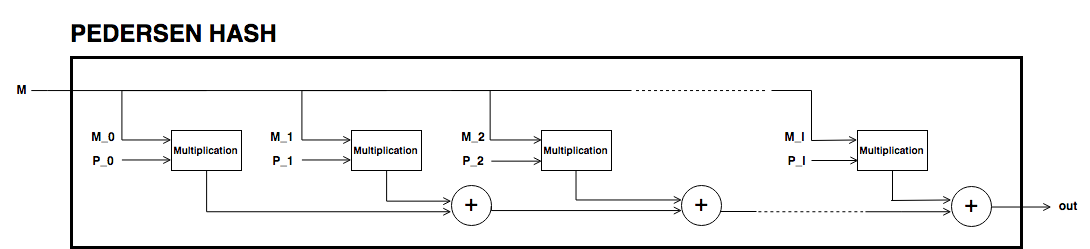
\includegraphics[scale=0.4]{figures/pedersen-hash.png}
	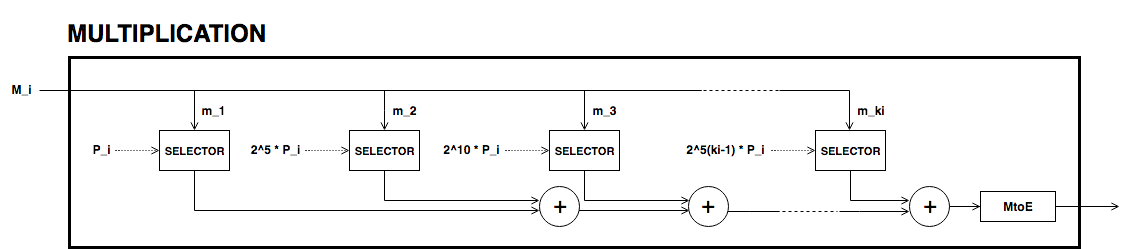
\includegraphics[scale=0.4]{figures/pedersen-multiplication.png}
\end{figure}

As the set of generators are fixed, we can precompute its multiples and use 4-bit lookup windows to select the right points. This is done as shown in the circuit called \textsc{selector}. This circuit receives 4-bit chunk input and returns a point. The first three bits are used to select the right multiple of the point and last bit decides the sign of the point. The sign determines if the $x$-coordinate should be taken positive or negative, as with Edwards curves, negating a point corresponds to the negation of its first coordinate. %[REF]. 

\begin{figure}[h]
	\centering
	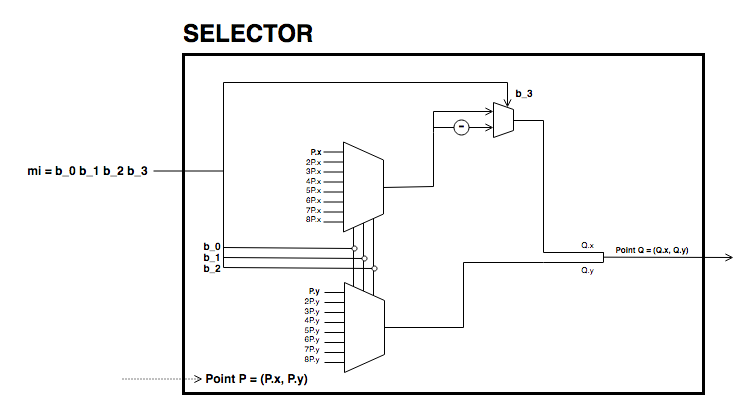
\includegraphics[scale=0.5]{figures/pedersen-multiplication-selector.png}
\end{figure}


		\label{sec-computation}
		\subsection{Examples And Test Vectors {\color{purple} Title Case}}
		
	\section{Challenges}
	% Challenges: for motivating the discussions, highlight the main challenges in creating such a standard,
% as well as any open or unresolved questions.
One of the main challenges to create this standard and to see it adopted by the community is
to provide correct, usable, and well-maintained implementations in as many languages as possible.

Some effort is also required to audit and verify code coming from the community
and claiming to implement the 4-bit window Pedersen hash function
to prevent the propagation of potentially insecure implementations.

Finally, the proposal as it stands today includes the padding of the message $M$ to a multiple of four bits.
There are potentials issues with this approach where collisions can happen.

%For example, the sequences of bits \texttt{10000} and \texttt{10000000} will share the same hash
%as the former pre-image is padded to \texttt{10000000} which is identical to the latter pre-image.
%We were unable to confidently solve this issue in time for the submission deadline of the first draft,
%but this oversight will be solve before the final version is submitted.




	\section{Security}
		\red{DIR QUE ESTEM A MONTGOMERY PERÒ QUE NO HI HA PROBLEMES: NO REPETIM PUNTS I NO SUMEM MAI EL 0. }
		\subsection{\color{purple} Overflow Prevention}
			As we described in section \ref{sec-computation}, 
%We have seen 
we use a windowed scalar multiplication algorithm with signed digits. Each 4-bit message chunk corresponds to a window called \textsc{selector} and each chunk is encoded as an integer from the set $\{-8..8\}\backslash \{0\}$. % and we allow to have up to $50$ windows. 
This allows a more efficient lookup of the window entry for each chunk than if the set $\{1..16\}$ had been used, because a point can be conditionally negated using only a single constraint \cite{sapling}.\\
% Sapling, the new network upgrade of Zcash, uses 3-bit windows but we propose to use 4-bit windows, as it requires less constraints per bit.\\

As there are up to 50 segments per each generator $P_i$, the largest multiple of the generator $P_i$ is $n\cdot P_i$ with 
$$n = 2^0 \times8 + 2^5 \times 8 + \left(2^5\right)^2 \times8 \dots + 	2^{245}\times 8 .$$
To avoid overflow, this number should be smaller than $(r-1)/2$. Indeed,
%We have to make sure that this number is smaller than $(r-1)/2$, where $r$ is the order of the large prime subgroup of the curve.  Indeed,
\begin{align*}
	\quad\; n 
	& = 8 \times \sum_{ k = 0}^{49} 2^{5k}
	= 8 \times \frac{2^{250}-1}{2^5-1}\\
	& = 466903585634339497675689455680193176827701551071131306610716064548036813064%\\
\end{align*}
\vspace{-0.2cm}
and 
\begin{align*}
	\frac{r-1}{2} &= 1368015179489954701390400359078579693038406986079283629600107830474223686520 \\
	& > n.\\ \vspace{0.4cm}
\end{align*}

			
	\section{Implementation}
		\subsection{A Note On Efficency {\color{purple} Moved as a subsection of Implementation by Jacques}}
			\subsection{Number Of Constraints Per Bit \red{-- canviar lleugerament la redacció!} {\color{purple} Title Case}}
			When using 3-bit and 4-bit windows, we have {{\bf 1 constraint for the sign}} and {{\bf 3 for the sum}} (as we are using the Montgomery form of the curve, that requires only 3). Now let's look at the constraints required for the multiplexers. \\

With 3-bit windows we need only one constraint per multiplexer, so {\bf 2 constraints} in total. \\

Standard 4-bit windows require two constraints: one for the output and another to compute $s_0*s_1$. So, a priori we would need 4 constraints, two per multiplexer. But we can reduce it to 3 as the computation of $s_0*s_1$ is the same in both multiplexers, so this constraint can be reused. This way only {{\bf 3 constraints}} are required. \\

So, the amount of constraints per bit are:
\begin{itemize}
	\item 3-lookup window : %\fbox{$s_0$}\fbox{$s_1$}\fbox{$s_2$} : 
		$ (1+3+2)/3 = 2 $ constraints per bit.
	\item 4-lookup window : %\fbox{$s_0$}\fbox{$s_1$}\fbox{$s_2$}\fbox{$s_3$} : 
		$ (1 +3+3)/4 = 1.75 $ constraints per bit. 
\end{itemize}

The specific constraints can be determined as follows: let the multiplexers of coordinates $x$ and $y$ be represented by the following look up tables:
\begin{table}[h]
    \begin{minipage}{.5\linewidth}
      \centering
	\begin{tabular}{c|c|c|c}
                $s_2$ & $s_1$ & $s_0$ & $out$\\
                	\hline
                	0 & 0 & 0 & $a_0$\\
                	0 & 0 & 1 & $a_1$\\
                	0 & 1 & 0 & $a_2$\\
                	0 & 1 & 1 & $a_3$\\
                	1 & 0 & 0 & $a_4$\\
                	1 & 0 & 1 & $a_5$\\
                	1 & 1 & 0 & $a_6$\\
                	1 & 1 & 1 & $a_7$
      	\end{tabular}
    \end{minipage}%
    \begin{minipage}{.5\linewidth}
      \centering
	\begin{tabular}{c|c|c|c}
		$s_2$ & $s_1$ & $s_0$ & $out$\\
		\hline
		0 & 0 & 0 & $b_0$\\
		0 & 0 & 1 & $b_1$\\
		0 & 1 & 0 & $b_2$\\
		0 & 1 & 1 & $b_3$\\
		1 & 0 & 0 & $b_4$\\
		1 & 0 & 1 & $b_5$\\
		1 & 1 & 0 & $b_6$\\
		1 & 1 & 1 & $b_7$
	\end{tabular}
    \end{minipage} 
\end{table}

\noi We can express them with the following 3 constraints:
% Then, we can express both multiplexers using the following 3 constraints:
\begin{itemize}
    \item 	$aux = s_0 s_1$ %(Reused for both multiplexers)
    \item 	$out = [ (a_7-a_6-a_5+a_4-a_3+a_2+a_1-a_0)*aux 
    		+ (a_6-a_4-a_2+a_0)*s_1$ \\
    		$\text{\qquad\;\;} + (a_5-a_4-a_1+a_0)*s_0
    		+ (a_4 - a_0) ] z 
    		+ (a_3-a_2-a_1+a_0)*aux + (a_2-a_0)*s_1 $\\
    		$\text{\qquad\;\;} + (a_1-a_0)*s_0+ a_0$
    \item	$ out = [ (b_7-b_6-b_5+b_4-b_3+b_2+b_1-b_0)*aux 
    		+ (b_6-b_4-b_2+b_0)*s_1$ \\
    		$\text{\qquad\;\;} + (b_5-b_4-b_1+b_0)*s_0 
    		+ (b_4 - b_0)] z 
    		+ (b_3-b_2-b_1+b_0)*aux + (b_2-b_0)*s_1 \\
    		\text{\qquad\;\:} + (b_1-b_0)*s_0+ b_0$\\
\end{itemize}

		\subsection{Existing Implementations}
			%	If relevant, submit an open source prototype implementation (by including a reference to the repository with the code).

% Others (entry?)
Nonce? of a claim?

Types of entries: claims, etc. D'una part en treiem el lloc on ho guardem i a l'altre etc.

	\section {Intellectual Property \red{-- Jordi} {\color{purple} Written by Jacques}}
		%	We aim to ensure that proposals can be freely implemented. Thus, proposals should disclose the existence of any known patents (awarded or pending) which may restrict free implementation. This may affect the decision process, and a detailed policy is being developed.

	% \newpage
	\addcontentsline{toc}{section}{References}
	\bibliographystyle{acm}
	\bibliography{lit}	

%\end{spacing}	
\end{document}
